%\documentclass[10pt]{article}
\usepackage{graphicx}
\usepackage{amssymb}
\usepackage{epstopdf}
\usepackage[]{epsfig}
\DeclareGraphicsRule{.tif}{png}{.png}{`convert #1 `basename #1 .tif`.png}

\textwidth = 7.0 in
\textheight = 9.5 in
\oddsidemargin = -0.25 in
\evensidemargin = 0.0 in
\topmargin = 0.0 in
\headheight = 0.0 in
\headsep = 0.0 in
\parskip = 0.05in
\parindent = 0.0in

\def \fdc    {{\textsc{fdc}}}

\begin{document}

\documentclass[10pt]{article}
\usepackage{graphicx}
\usepackage{amssymb}
\usepackage{epstopdf}
\usepackage[]{epsfig}
\DeclareGraphicsRule{.tif}{png}{.png}{`convert #1 `basename #1 .tif`.png}

\textwidth = 7.0 in
\textheight = 9.5 in
\oddsidemargin = -0.25 in
\evensidemargin = 0.0 in
\topmargin = 0.0 in
\headheight = 0.0 in
\headsep = 0.0 in
\parskip = 0.05in
\parindent = 0.0in

\def \fdc    {{\textsc{fdc}}}

\begin{document}



\section*{Data Acquisition (DAQ)}


\subsubsection*{Overview}

The GlueX data acquisition system must:
\begin{itemize}
\item support a deadtimeless front-end system at a 200 kHz L1 trigger rate
\item collect data from the front-end modules at 1 GB/s
\item build event fragments into a single event record
\item pass built events to a level 3 farm
\item write level 3 accepted events to mass storage at 100 MB/sec
\item deliver a small subset of the events to online calibration and
  monitoring systems
\end{itemize}

GlueX expects to fill approximately 70-80 readout crates 
containing 25,000 channels of electronics. 
We expect a level 3 reduction of 90\%, which reduces the 1 GB/s raw
rate to an accepted event data rate to disk of around 100 MB/s.

GlueX will use CODA, the standard data acquisition system developed at
JLab, but at higher trigger and data rates than have been achieved so far.
We note that the high rate makes it impossible to interrupt the front-end
processors for every event. Use of fully-pipelined digitizing electronics
will be necessary.  To manage a 1 GB/s data rate from the front-end to L3
a staged, parallel event building scheme will also be required. Finally,
we note that CODA has not been run with an integrated high-rate level 3 farm.

\subsubsection*{Stage One R\&D}

There are several parallel R\&D efforts that need to take place to
establish first the feasability of the full system and then support for
the staged detector prototyping efforts that will take place over the
course of the next few years. Near term R\&D efforts must also take into
consideration the existing 6 GeV program and provide a smooth upgrade path
for the running experiments.

The DAQ group is involved jointly with the JLAB electronics group in the 
development of the 10-bit 250 MHz flash ADC design. This module should be
completed and will be used with the F1TDC to define a fully pipelined front
end to interface with GlueX detector subsystems. These modules can also be
used in the existing experimental Halls. Addional hardware support for the 
pipelined systems should include the design of a new VME trigger interface 
board, and a prototype (for small numbers of crates) trigger/clock 
distribution system (See the GlueX Electronics for DAQ plan for details). 

Software R\&D include the development of a new CODA Readout Controller
(ROC) component that will run on either an Embedded Linux or VxWorks
operating system resident on VME Based Single board computers. This
component provides the interface with the CODA backend system and the
first stage for parallel event-building support. Software libraries for 
the access, programming, readout, and monitoring of the pipelined 
electronics will have to be developed.

Proof of principle for a network-based staged parallel Event Builder
consisting of a variable number of network nodes and capable of sustaining
an aggregate throughput of over 1 GB/s should be established early on. For
this purpose a small DAQ processor farm (~30 nodes) is being assembled. A
prototype Event Builder system will be designed around the existing CODA ET
(Event Transport) system. 

An Experiment Control system integrating DAQ Run Control with slow
controls is being developed using a JAVA framework with distributed
intelligent ``Agents'' monitoring and controlling the various components
and subsystems. The User will be able to describe the system and its
behaviors through an ontology language (COOL) that the agents understand.
 

\subsubsection*{Goals and Milestones}

The first stage of the DAQ farm is expected to be installed by February
2006 in the new wing of Cebaf Center. Software development of the ROC,
event builder, and run control will continue throughout the year with
working models for all expected by the end of 2006. 

The high speed FADC is expected to be in prototype by the summer or early 
Fall of 2006, and from that stage library support can begin to be developed and
tested. The new VME trigger interface capable of supporting both the old
trigger supervisor as well as the new pipelined front-end should be
prototyped roughly within the same time frame. This hardware too will need software
support developed for it. 

The extension of providing a new trigger (and clock) distribution system 
will be difficult to fully specify before the end of 2006 and is somewhat
dependent on parallel electronics developments (in conjunction with the
electronics group) using the VXS switched serial extension to VME (VITA 41). 
One could optimistically hope to prototype something by mid 2007.

By early 2007 there should be enough hardware and software development to
support small detector system prototyping, and beam tests that would
encompass the core functionality of the GlueX DAQ system. 


\subsubsection*{Personnel}

Primary responsibility for developing CODA belongs to the DAQ group at
JLab.  This includes both hardware and software development The DAQ group
staffing is currently five full time (D. Abbott, E. Wolin, C. Timmer,
V. Gyurjyan, and E. Jastrzembski) and one part-time (D. Lawrence) FTE. DAQ hardware
development (managed by E. Jastrzembski) is highly dependent on
availability of additional engineering support from the Physics Electronics group.

There is a request for one additional DAQ group member to help primarily in the development
of the DAQ farm and parallel Event Building R\&D. Additional support could be used in the
development of driver libraries, diagnostics, and utilities for all of the new DAQ electronics
hardware being designed.



\begin{figure}[p]
\begin{center}
\includegraphics[height=15cm]{GluexDAQ.eps}
\caption{Schematic of the GlueX data acquisition system and specific
subsystems. Event and data rates are indicated at the various stages.
\label{fig:plan}}
\end{center}
\end{figure}



\end{document} 
